\documentclass[12pt, a4paper]{report}
\usepackage[top=1.0in, bottom=1.0in, left=0.8in, right=0.8in]{geometry}
\usepackage{graphicx}
\usepackage{amsmath}
\usepackage{listings}
\usepackage{fancyvrb}

 	
\title{\textbf{EE2703 : Applied Programming Lab \\ Assignment 4 \\ Fourier Approximations}} 
\author{Aditya Nanda Kishore\\ EE20B062} 

\date{\today} % Date for the report

	
\begin{document}		
\maketitle
\section{Abstract}
The aim of this assignment is to understand how any function can be represented as a sum of periodic trigonometric functions, forming \textit{Fourier coefficients} through \textit{Integration} as well as \textit{Least Square Method} and the checking the accuracy of the newly formed functions.



\section{Introduction}
We are given two functions $cos(cos(x))$, $e^x$  and we have to represent these two functions as fourier series over the interval (0, 2$\pi$) 
given by \newline

\large

\begin{equation}
a_0 + \sum_{n=1}^{\infty} (a_n cos(nx) + b_n sin(nx))
\end{equation}

\normalsize
We need to
\begin{itemize}
	\item Find Fourier Coefficients through Integration and plot them
	\item Find Fourier Coefficients through Least Square Method and plot them
	\item Compare the results
\end{itemize}
\section{Assignment}
\subsection{Q1}
% When adding * to \section, \subsection, etc... LaTeX will not assign
% a number to the section
Importing the standard libraries
\begin{Verbatim}
from pylab import *
import numpy as np
import matplotlib.pyplot as plt
import scipy.integrate as integrate
\end{Verbatim}

The code here generates two functions for either a scalar/vector input and returns scalar/vector output.   

\begin{Verbatim}
def cos_cos(x):
    y = np.cos(np.cos(x))
    return y

def exp(x):
    y = np.exp(x)
    return y
\end{Verbatim}

Now we plot these both functions over the interval $ [-2\pi, 4\pi)$ and see that $cos(cos(x))$ is a periodic function with the period $\pi$ and $e^x$ isn't periodic.But for this question, we are considering $e^x$ to be periodic with period $2\pi$

\begin{Verbatim}

x = np.arange(-2*np.pi, 4*np.pi, 0.01)
M_0 = np.array(cos_cos(x))
M_1 = np.array(np.log(exp(x)))
M = np.vstack((M_0,M_1)).T
plt.plot(x, M_0)
plt.xlabel('x')
plt.legend(['cos(cos(x))'])
plt.grid()
plt.show()

plt.plot(x, M_1)
plt.xlabel('x')
plt.legend(['log(exp(x))'])
plt.grid()
plt.show()


\end{Verbatim}


\begin{figure}[!tbh]
   	\centering
   	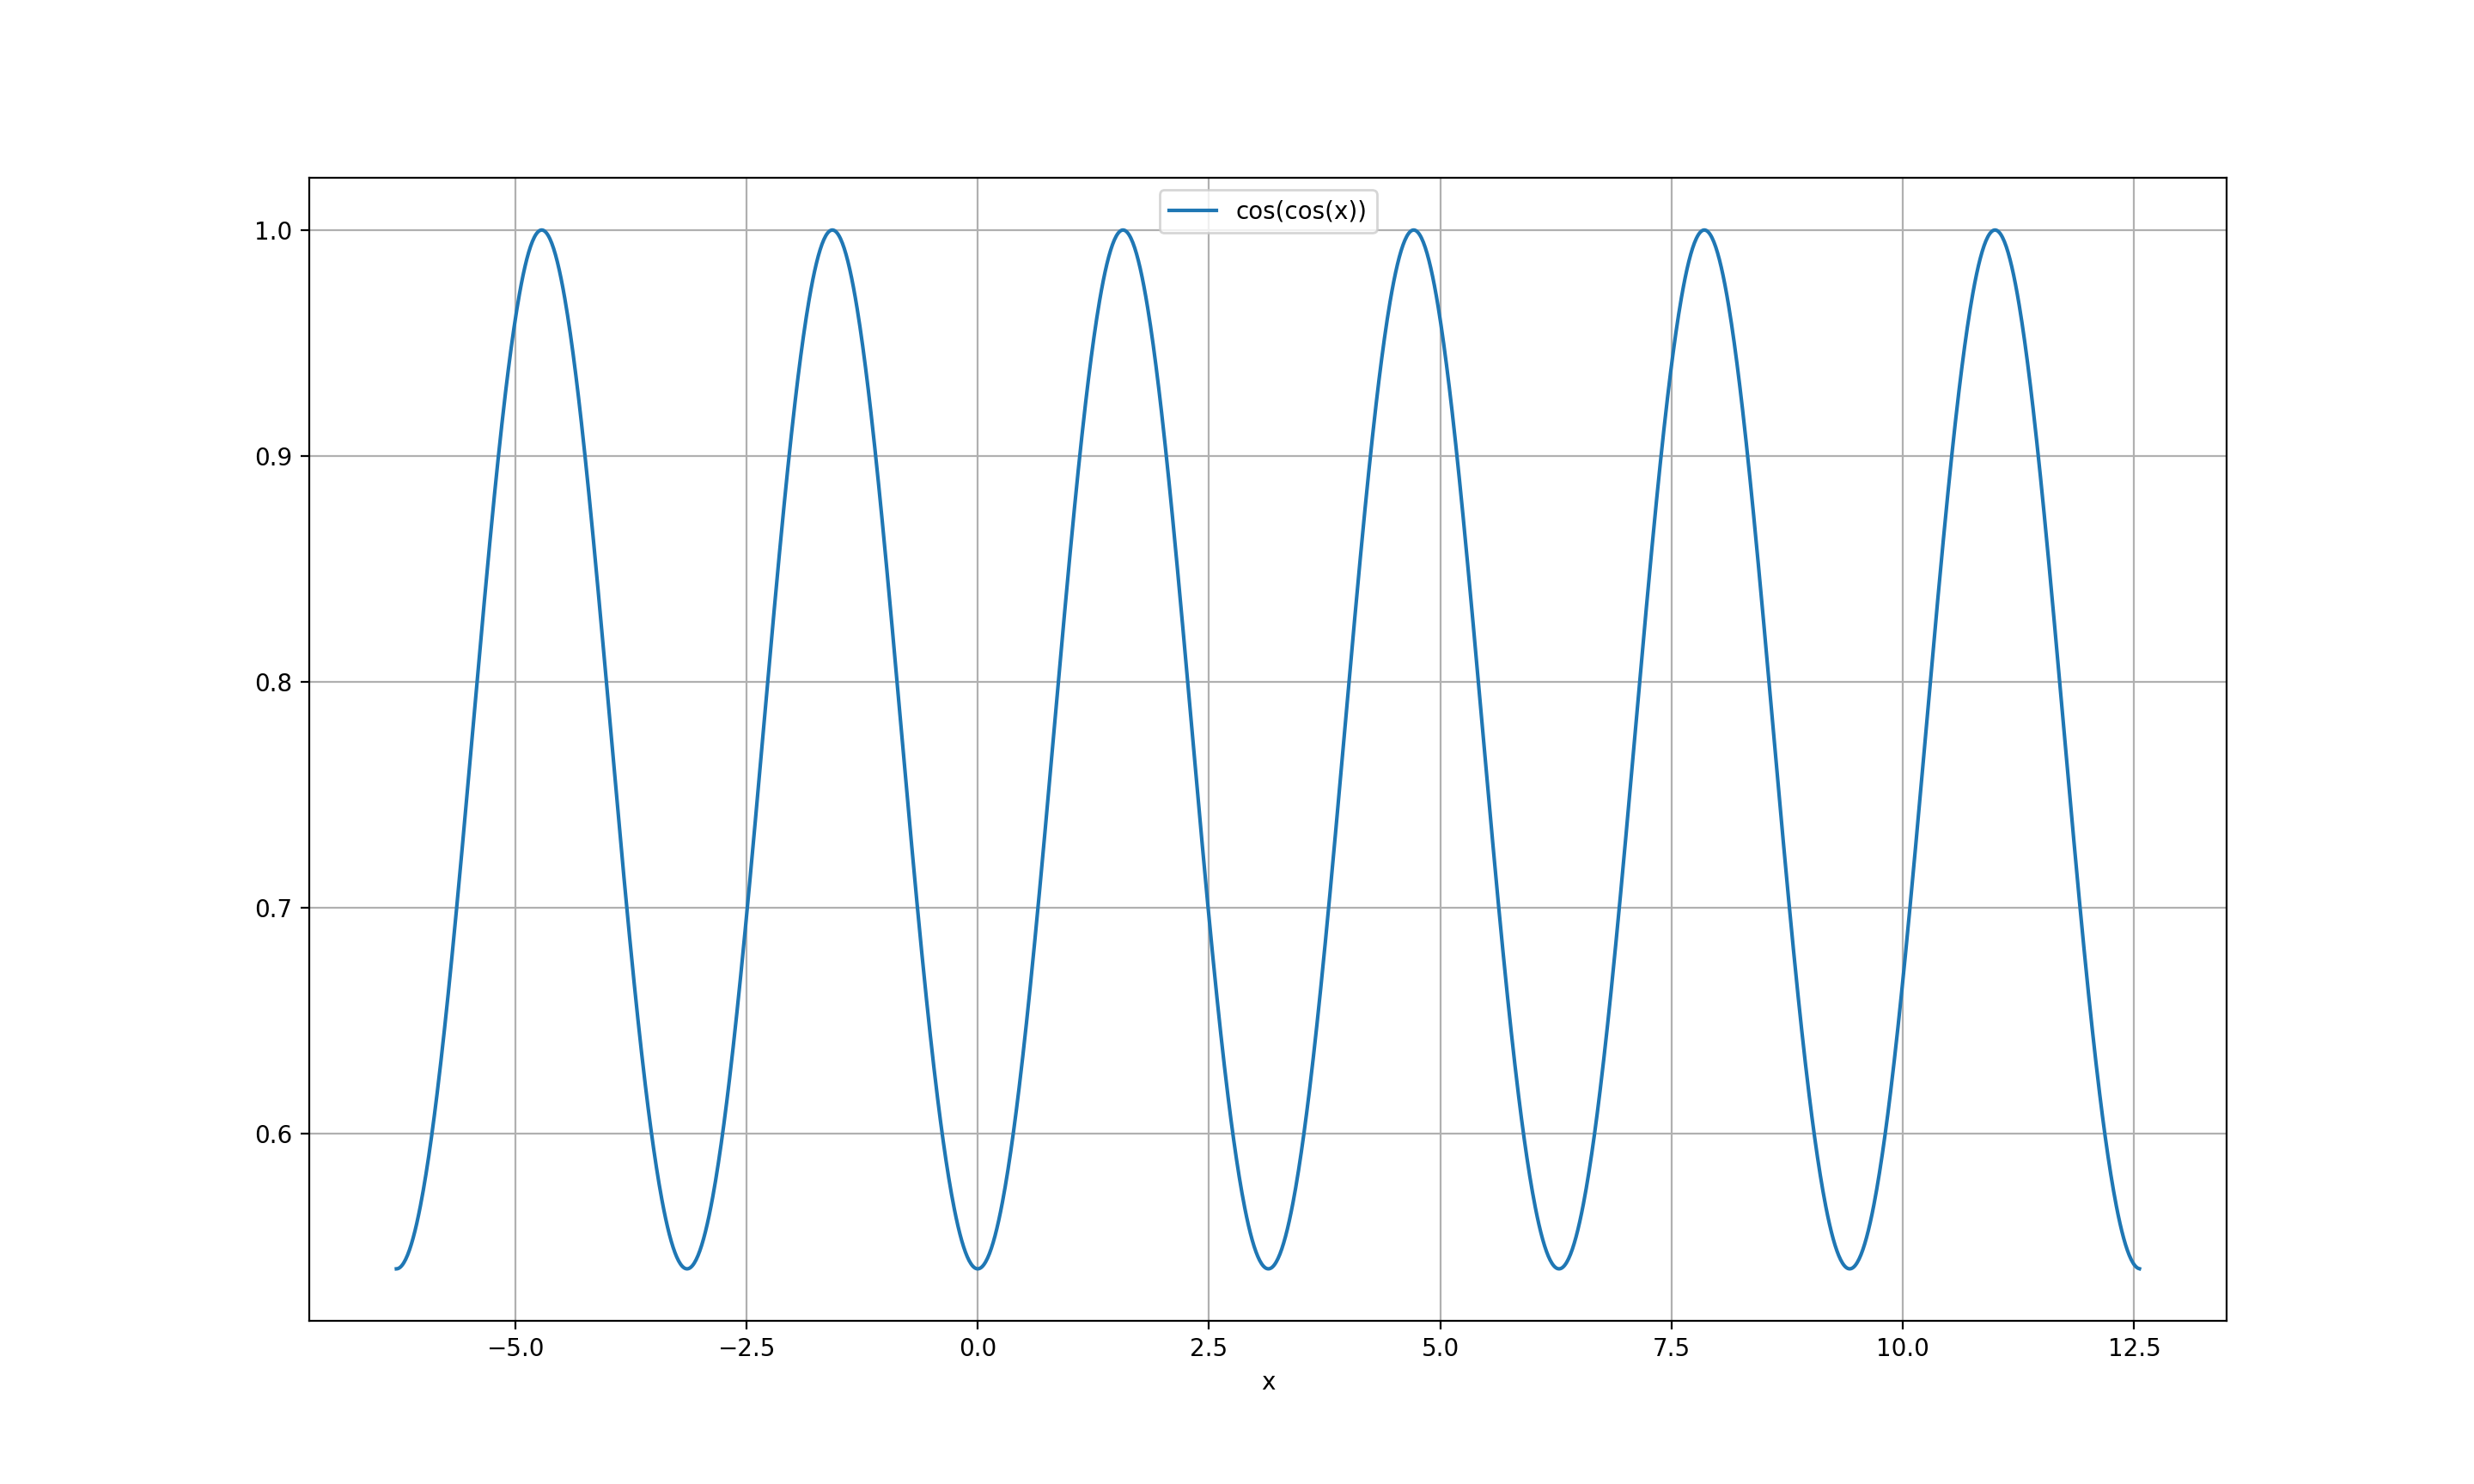
\includegraphics[scale=0.25]{Q1.png}
   	\caption{Double Cosine Function}
   	\label{fig:allgraphs}
   \end{figure} 


 \begin{figure}[!tbh]
   	\centering
   	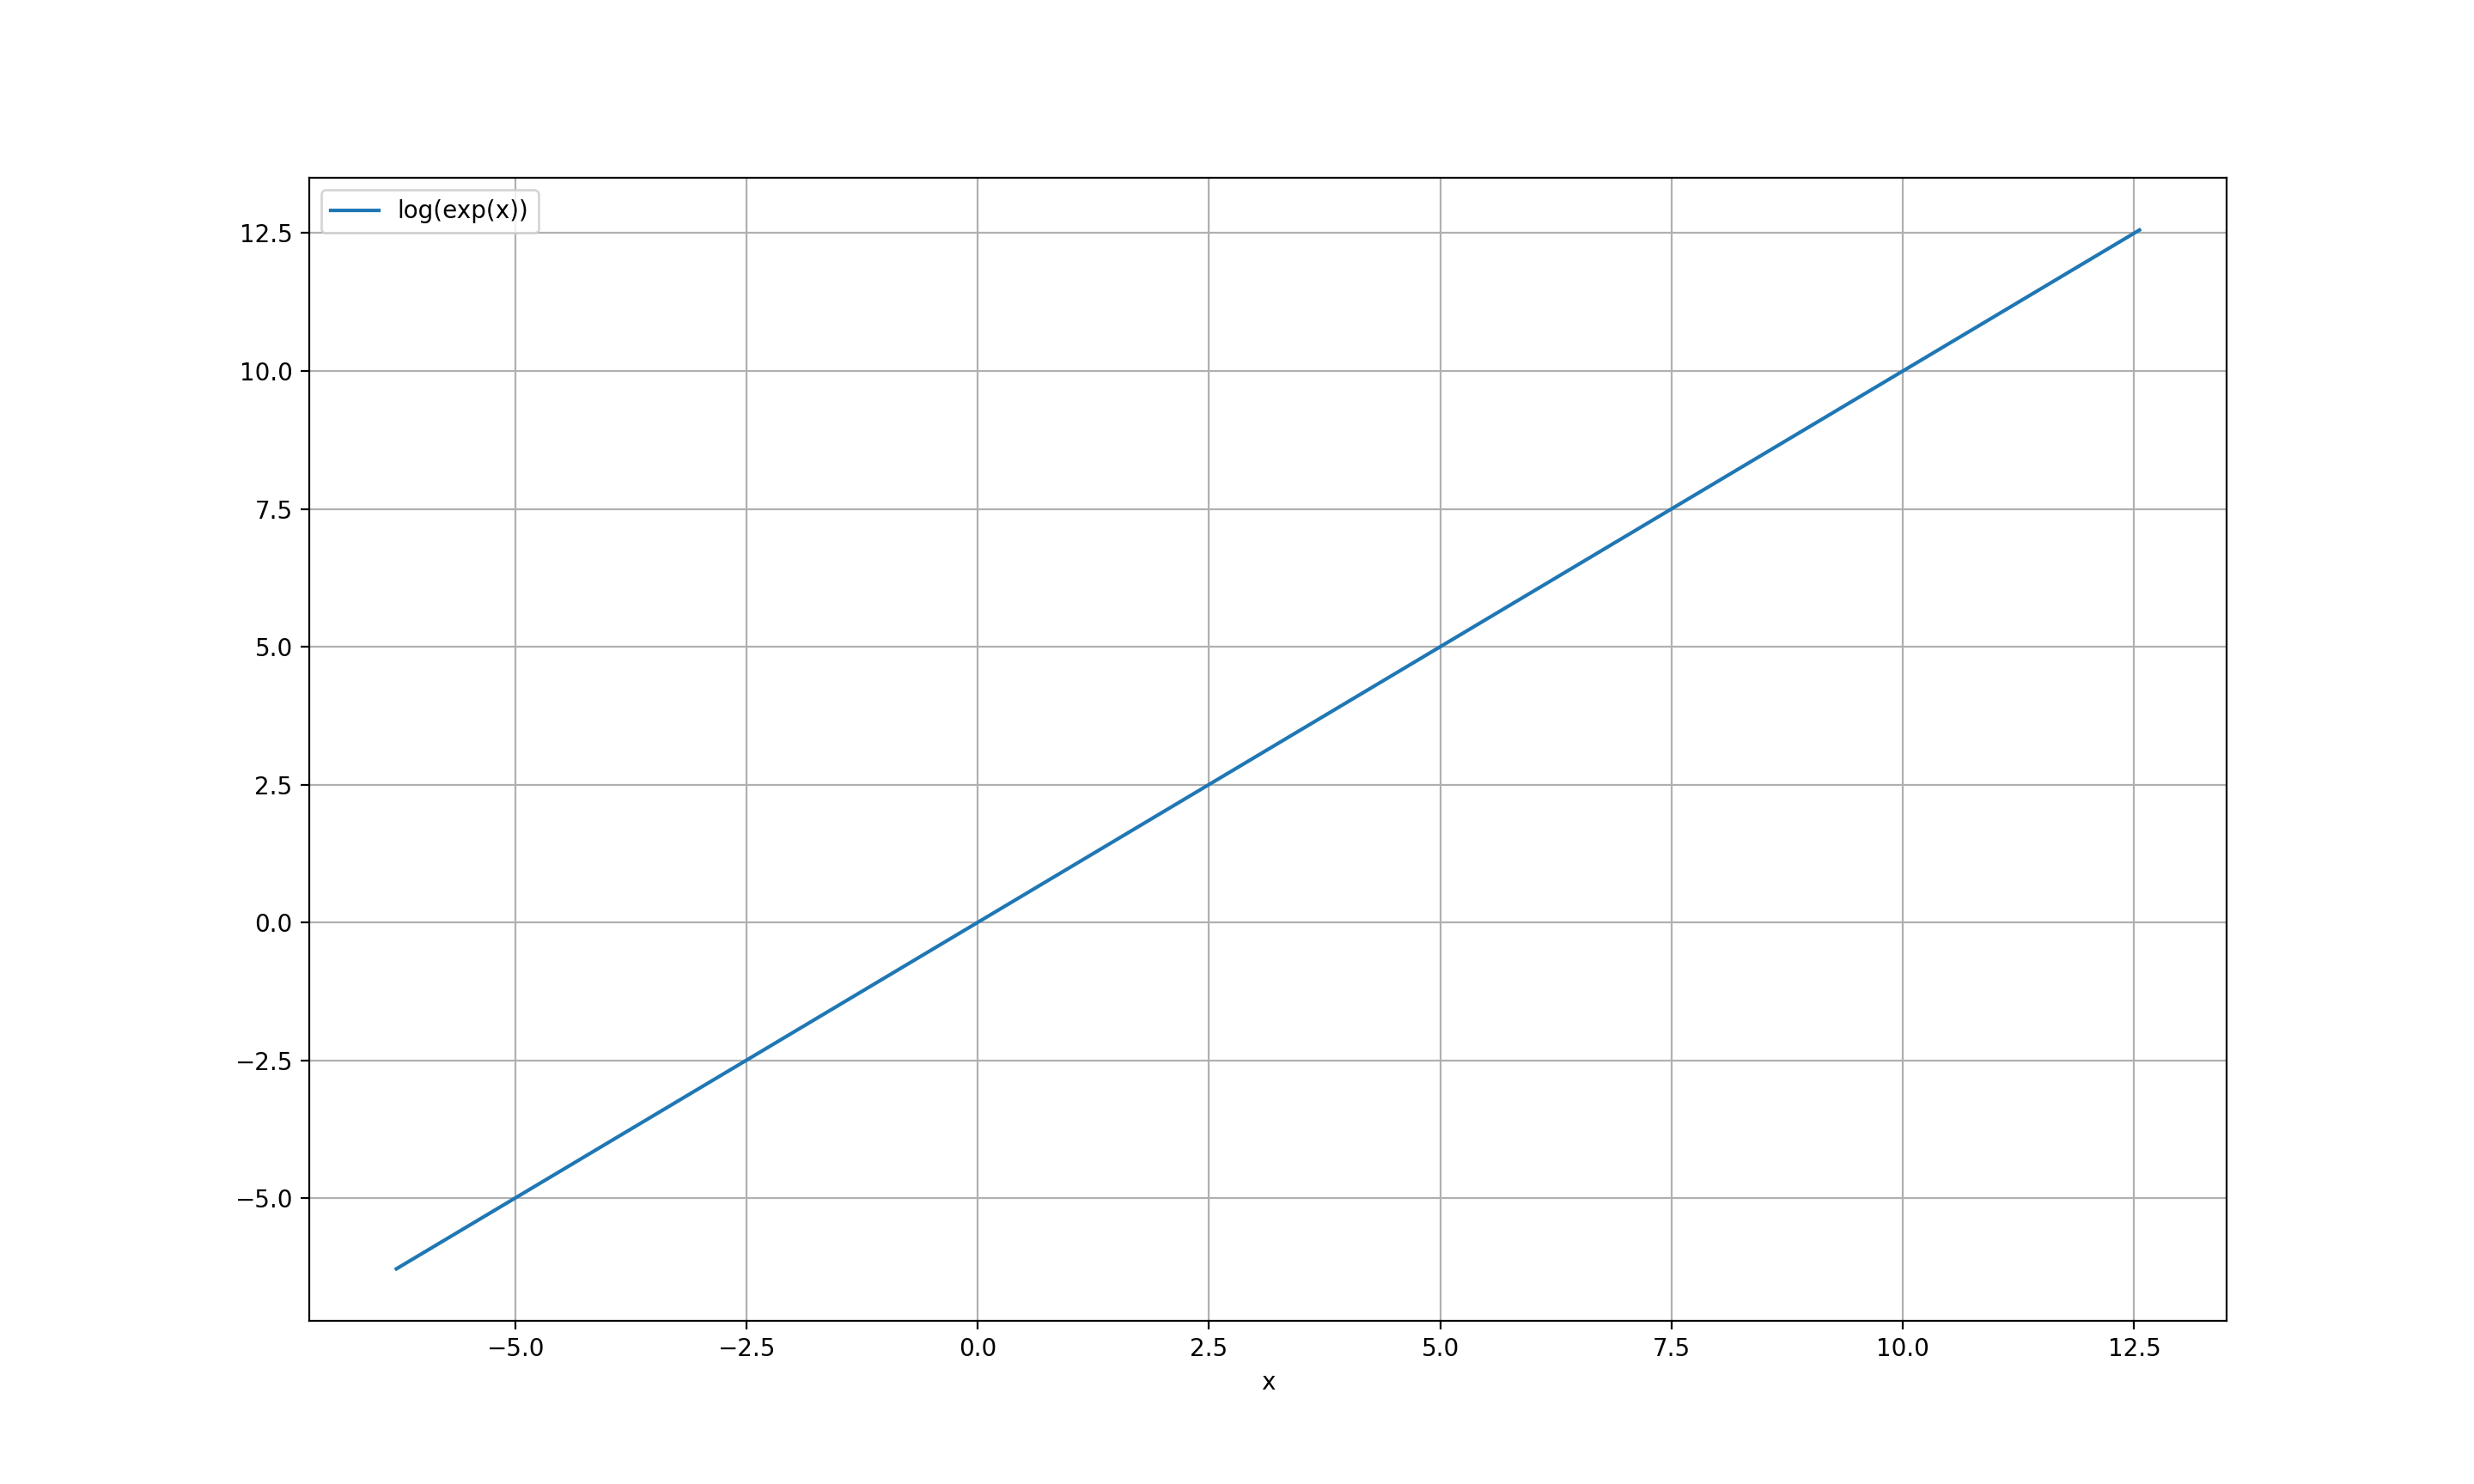
\includegraphics[scale=0.25]{Q1b.png}
	\caption{Exponential Function(Semilog Graph)}
   	\label{fig:trueNoMatrix}
 \end{figure}

If we look at the fourier series, we can clearly see that it is only going to represent periodic functions.So the function here we are considering is actually a periodic function with period $2\pi$ and behaves like the actual function in $ [0,2\pi) $
 \subsection{Q2}
Now we are going to obtain the coefficients through integration. The formulae for coefficients is 

\begin{figure}[!tbh]
   	\centering
   	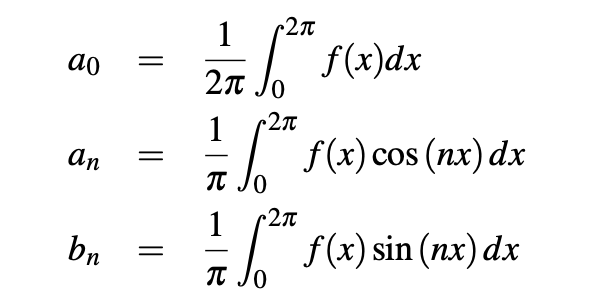
\includegraphics[scale=0.75]{1.png}
   	\label{fig:errorbars}
\end{figure}

Implementing the code for the above formulae

\begin{Verbatim}
def coefficents_find(f):

    def u(x,k):
        return f(x)* np.cos(k*x)
    def v(x,k):
        return f(x)* np.sin(k*x) 
    a = []
    a0 = (1/( 2* np.pi)) * (integrate.quad(u , 0, 2* np.pi, args = 0))[0]
    a.append(a0)
    for i in range(1,26):
        a.append((1/np.pi) * integrate.quad(u, 0, 2*np.pi, args= i)[0]) 
        a.append((1/np.pi) * integrate.quad(v, 0, 2*np.pi, args= i)[0])
    return a

\end{Verbatim}

This code returns the first 25 fourier coefficients of any function that's given as the input in the given format as in part 3. We, in the next part calculate the 25 coefficients for $cos(cos(x))$, $e^x$.
   
 \subsection{Q3}
 
 First We split the array we got in Q2 into two sub arrays and plot them separately with respect to n.This is to plot two consecutive elements in the array under same n. Here we plot the coefficients found in a semilog graph and a log-log graph in red circles vs n.
 \begin{Verbatim}
 
arr_1 = np.array(coefficents_find(cos_cos))
arr_1a = []
arr_1b = []
arr_1a.append(arr_1[0])
for i in range(1,len(arr_1)):
    if i%2 == 0:
        arr_1b.append(arr_1[i])
    else:
         arr_1a.append(arr_1[i])


arr_2 = np.array(coefficents_find(exp))
arr_2a = []
arr_2b = []
arr_2a.append(arr_2[0])
for i in range(1,len(arr_2)):
    if i%2 == 0:
        arr_2b.append(arr_2[i])
    else:
         arr_2a.append(arr_2[i])
n1 = np.arange(0,26)
n2 = np.arange(1,26)

fig, axs = plt.subplots(2)
fig.suptitle('Semilog Plots of First 25 Fourier Coefficients')
axs[0].semilogy(n1, np.abs(arr_1a), 'ro')
axs[0].semilogy(n2, np.abs(arr_1b), 'ro')
axs[0].set_title("Cos(Cos(x))")
axs[0].grid()


axs[1].semilogy(n1, np.abs(arr_2a), 'ro')
axs[1].semilogy(n2, np.abs(arr_2b), 'ro')
axs[1].set_title("exp(x)")
axs[1].grid()


plt.show()

fig, axs = plt.subplots(2)

fig.suptitle('Log-log Plots of First 25 Fourier Coefficients')
axs[0].loglog(n1, np.abs(arr_1a), 'ro')
axs[0].loglog(n2, np.abs(arr_1b), 'ro')
axs[0].set_title("Cos(Cos(x))")
axs[0].grid()
axs[0].legend(['a', 'b'])

axs[1].loglog(n1, np.abs(arr_2a), 'ro')
axs[1].loglog(n2, np.abs(arr_2b), 'ro')
axs[1].set_title("exp(x)")
axs[1].grid()

plt.show()

\end{Verbatim}

I used subplots to plot the graph , because it made comparison easier. These are the results I got

\begin{figure}[!tbh]
   	\centering
   	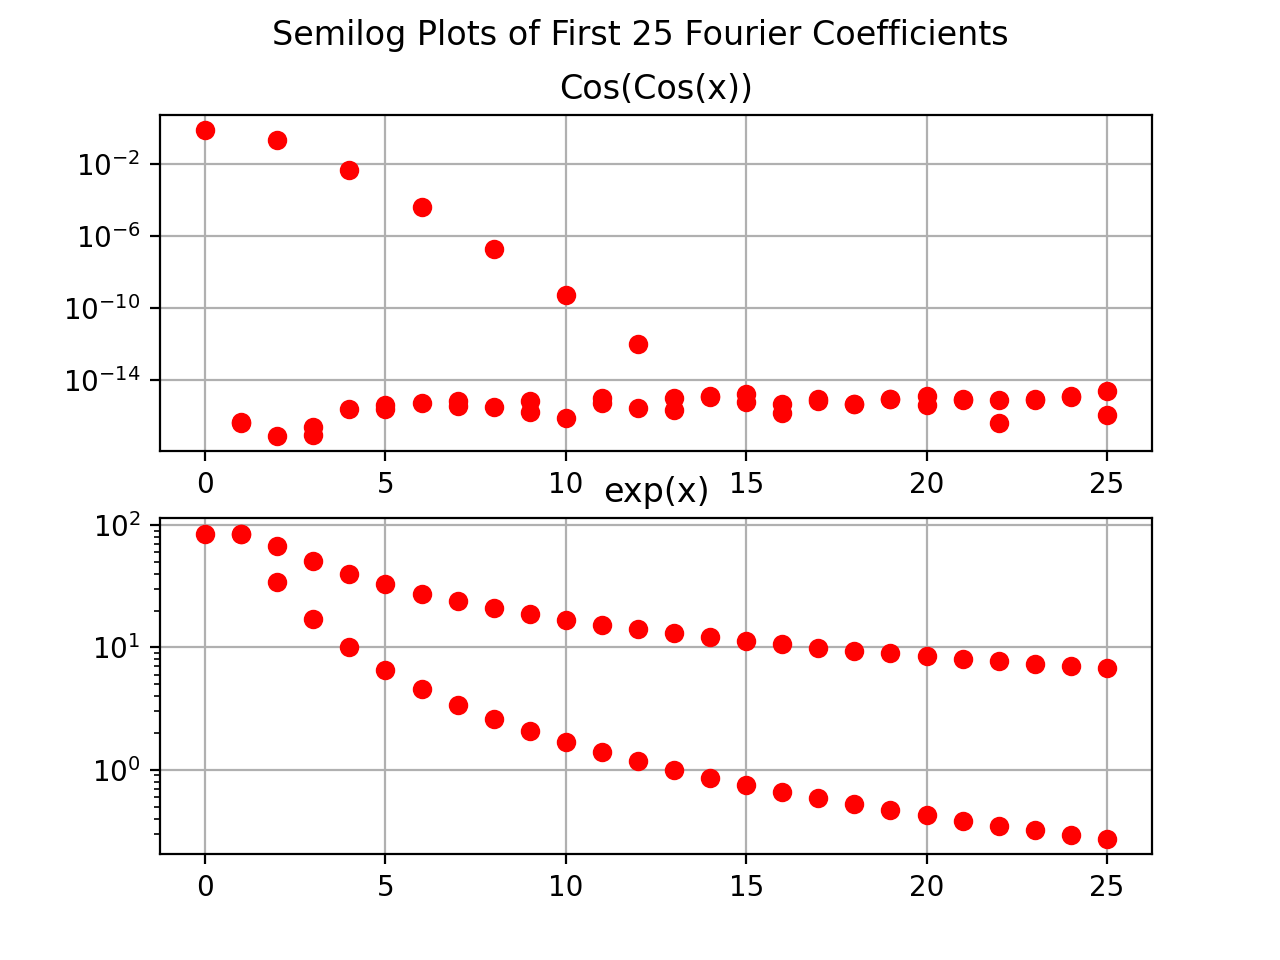
\includegraphics[scale=0.75]{Q3a.png}
	\caption{Semilog Plots}
   	\label{fig:trueMatrix}
   \end{figure}

\begin{figure}[!tbh]
   	\centering
   	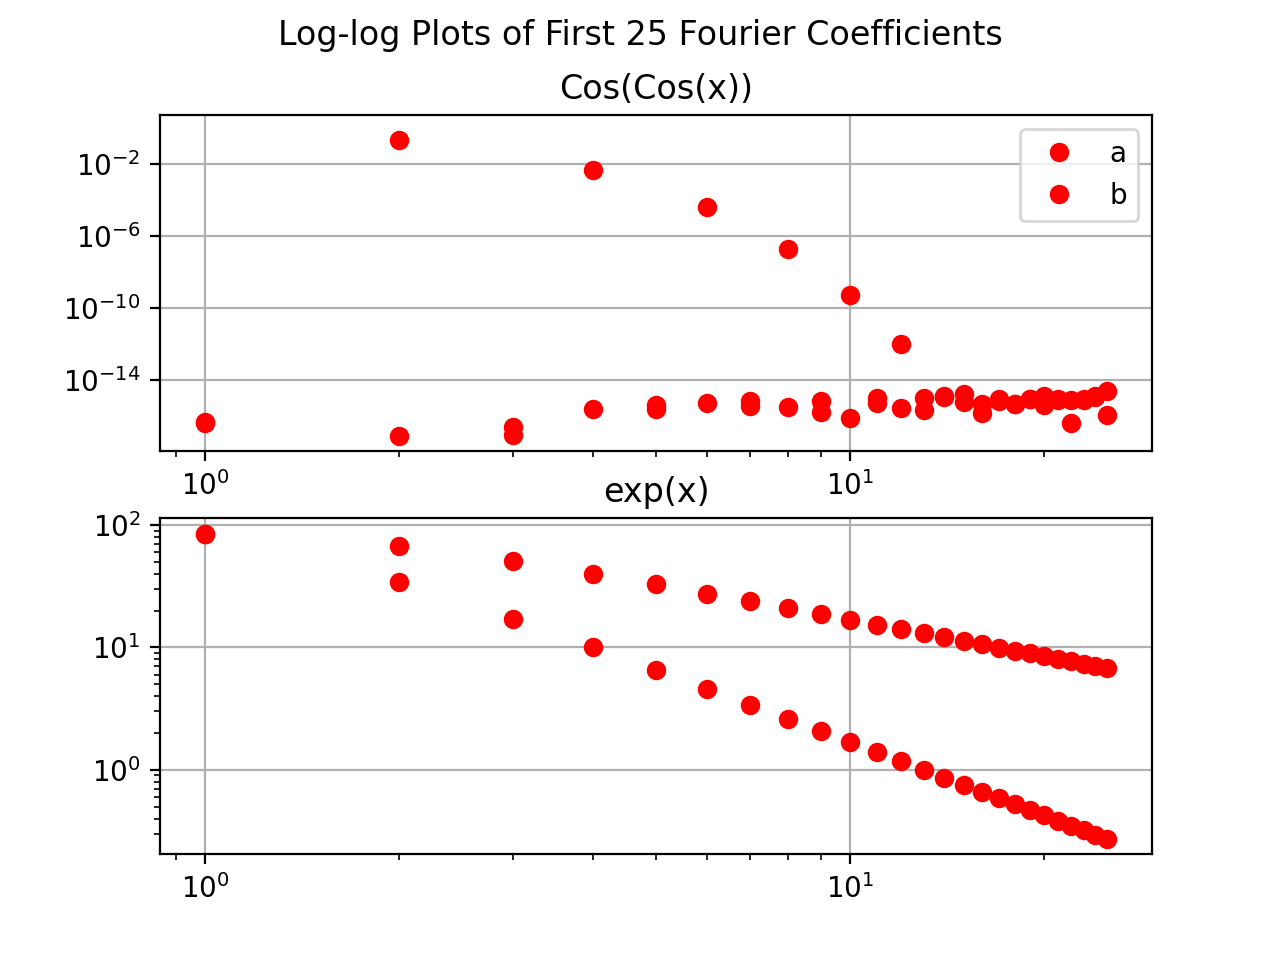
\includegraphics[scale=0.75]{Q3b.png}
	\caption{log-log plots}
   	\label{fig:trueMatrix}
   \end{figure} 
(a)  $b_n$ for $cos(cos(x))$ is given by\newline

\[ b_n= \int_{0}^{2\pi} cos(cos(x)) sin(nx) \,dx \]
\[ b_n= \int_{0}^{2\pi} cos(cos(2\pi-x)) sin(n(2\pi-x)) \,dx \]
\[ b_n= \int_{0}^{2\pi} -cos(cos(x)) sin(nx) \,dx \]
this implies
$b_n = -b_n$
Hence, $b_n = 0$

Hence, the values we found are very close to zero\newline

(b) When we look at the coefficients of second function, The formula is 
\begin{equation}
a_n  = {1\over 2\pi}\int_{0}^{2\pi} e^x cos(nx) \,dx 
\end{equation}

We know that,
\begin{equation}
\int {e^{ax}cos(bx)} = {e^{ax}\over{a^2 + b^2}}(b sin(bx) + a cos(bx)) +c
\end{equation}

So,
\begin{equation}
 {1\over 2\pi}\int_{0}^ {2\pi} {e^{x}cos(nx)} =  {1\over 2\pi} {e^{x}\over{1 + n^2}}(n sin(nx) + cos(nx))
\end{equation}

Hence, $a_n$ here is proportional to ${1\over{1+n^2}}$ and this will be the case for $b_n$ too and the actual function isn't periodic and sinusoidal too. So it's difficult to accurately reach the function with less number of frequencies. So the frequency spectrum is broader for the former.Whereas in the case of double cos, The Fourier transform would yield something like this, clearly saying that after very less number of frequencies the strength of the spectrum is almost zero.Since it's a sinusoidal, less number of frequencies would give us the actual function accurately. This is also reason for one of the further questions, where we get a lot of deviation by using least square method for $e^x$\newline

(c) Since $a_n$ and $b_n$ for $e^x$ are proportional to ${1\over{1+n^2}}$ ,  $log({1\over{1+n^2}})$ can be approximated to $-2logn$ which is proportional to $logn$ in turn. Hence log-log plot is approximately linear. Now , For the Semilog plot of $cos(cos(x))$, since it's almost exponential, $log{a_n}$ is proportional to n. Hence, Semilog plot of double cosine function is linear.
   


 \subsection{Q4 and Q5}
 Now, we are going to use Least Square Methods to find coefficients. We are creating two matrices here as shown below and then using \textit{lstsq} to find the coefficients. But these coefficients aren't accurate and the function formed from this function will highly deviate from the actual function. So I am forming a vector with the actual function values and a matrix with trigonometric coefficients using a for loop which iterates 25 times and amends the matrix.
 
 
\begin{figure}[!tbh]
   	\centering
   	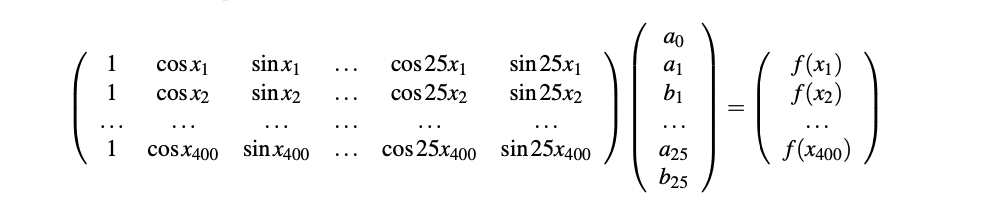
\includegraphics[scale=1]{3.png}
   	\label{fig:sample}
   \end{figure}
   
   
 \begin{Verbatim}
x = linspace(0, 2*np.pi, 401)
x = x[:-1]
b = cos_cos(x)
A=np.zeros((400,51)) 
A[:,0]=1
for k in range(1,26):
        A[:,2*k-1]=np.cos(k*x)
        A[:,2*k]=np.sin(k*x)

c_double_cos = np.linalg.lstsq(A,b, rcond = None)[0]
\end{Verbatim}

After this, we have to plot the coefficients and compare them with the previous coefficients. To differentiate the new points, They are plotted in green circles.For plotting I am again splitting the array and then plotting just like in Q3

\begin{Verbatim}
c_double_cosa = []
c_double_cosb = []
c_double_cosa.append(c_double_cos[0])
for i in range(1,len(c_double_cos)):
    if i%2 == 0:
        c_double_cosb.append(c_double_cos[i])
    else:
         c_double_cosa.append(c_double_cos[i])


b = exp(x)
c_exp = np.linalg.lstsq(A,b, rcond = None)[0]
c_expa = []
c_expb = []
c_expa.append(c_exp[0])
for i in range(1,len(c_exp)):
    if i%2 == 0:
        c_expb.append(c_exp[i])
    else:
         c_expa.append(c_exp[i])

fig, axs = plt.subplots(2)
fig.suptitle('Semilog Plots of First 25 Fourier Coefficients')
axs[0].semilogy(n1, np.abs(arr_1a), 'ro')
axs[0].semilogy(n2, np.abs(arr_1b), 'ro')
axs[0].semilogy(n1, np.abs(c_double_cosa), 'go')
axs[0].semilogy(n2, np.abs(c_double_cosb), 'go')
axs[0].set_title("Cos(Cos(x))")
axs[0].grid()


axs[1].semilogy(n1, np.abs(arr_2a), 'ro')
axs[1].semilogy(n2, np.abs(arr_2b), 'ro')
axs[1].semilogy(n1, np.abs(c_expa), 'go')
axs[1].semilogy(n2, np.abs(c_expb), 'go')
axs[1].set_title("exp(x)")
axs[1].grid()

plt.show()
\end{Verbatim}


\begin{figure}[!tbh]
   	\centering
   	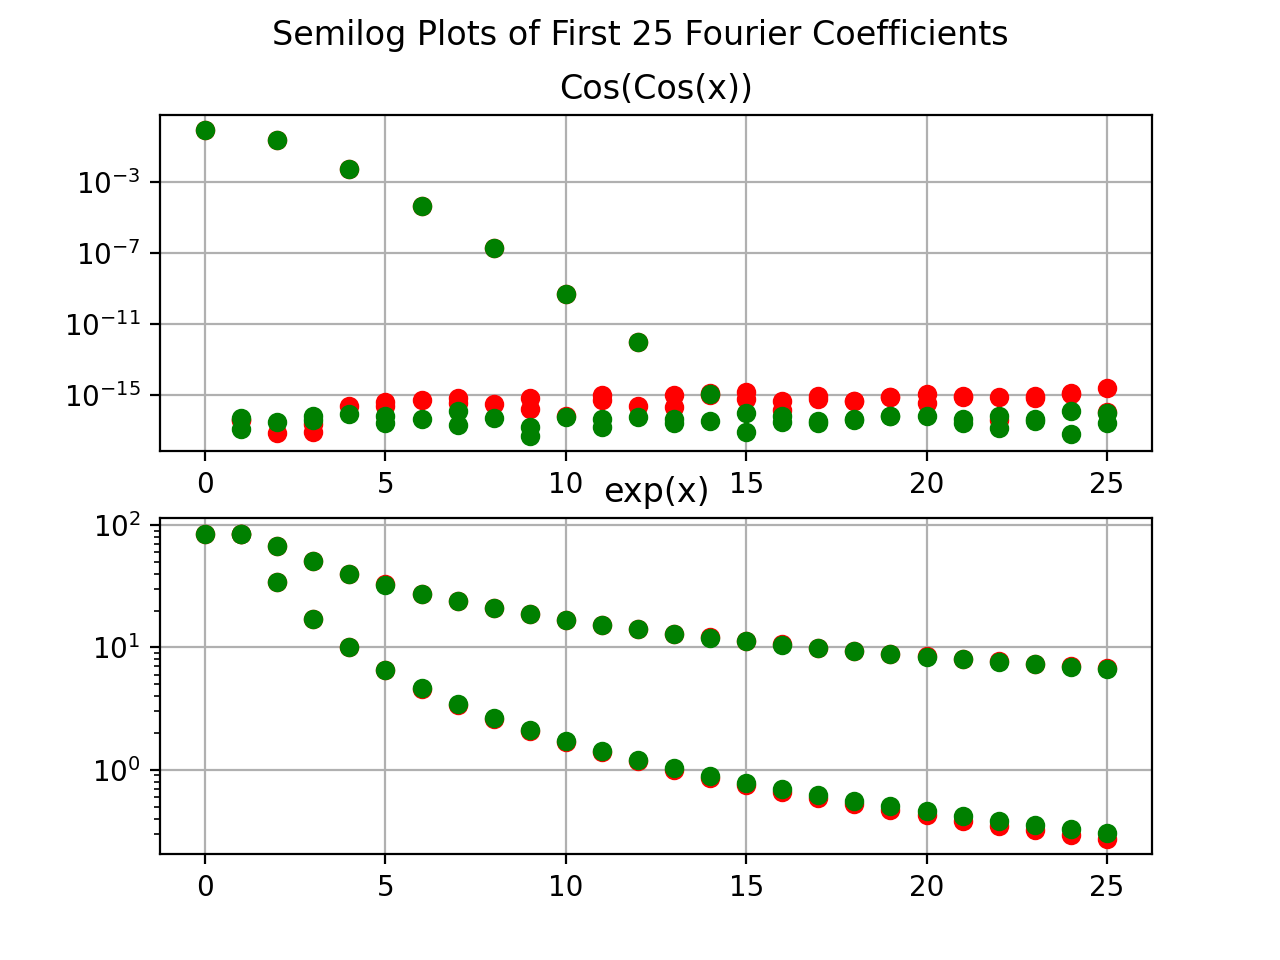
\includegraphics[scale=0.75]{Q5.png}
   	\caption{Coefficients with lstsq vs Coefficients with Integration}
   	\label{fig:sample}
   \end{figure}
  
 We can see that Coefficients are exactly matching for the second plot whereas almost matching for the first plot
 
 \subsection{Q6}
No, The coefficients formed with both the methods are not same. We can see the difference here. This is because the least squares method assumes no other frequency above n = 25 contributes to the function, but that's not the case here.
 
 \begin{Verbatim}


\end{Verbatim}

\begin{figure}[!tbh]
   	\centering
   	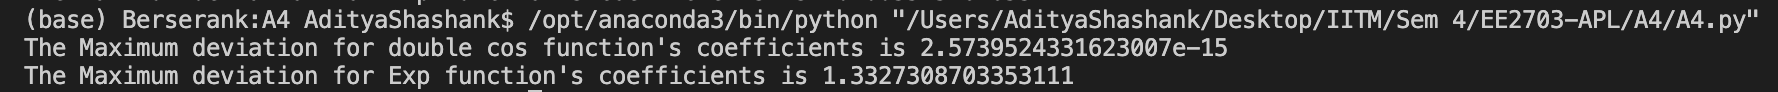
\includegraphics[scale=0.5]{4.png}
   	\caption{Contour Plot of $\epsilon_{ij}$}
   	\label{fig:sample}
   \end{figure}


 \subsection{Q7}
 Now we calculate the function values with the new coefficients and plot it in green and the old function which is the actual function in red. We can see that $cos(cos(x))$ is perfectly matching whereas $e^x$ isn't.
 
  \begin{Verbatim}
  
approx_double_cos = A. dot(c_double_cos)
approx_exp = A. dot(c_exp) 

fig, axs = plt.subplots(2)
fig.suptitle('Comparison of two functions')

axs[0].semilogy(x, cos_cos(x), 'ro')
axs[0].semilogy(x, approx_double_cos, 'go')
axs[0].set_title("Cos(Cos(x)) Comparison")
axs[0].grid()

axs[1].semilogy(x, exp(x), 'ro')
axs[1].semilogy(x, approx_exp, 'go')
axs[1].set_title("Exp(x) Comparison")
axs[1].grid()
plt.show()

\end{Verbatim}


\begin{figure}[!tbh]
   	\centering
   	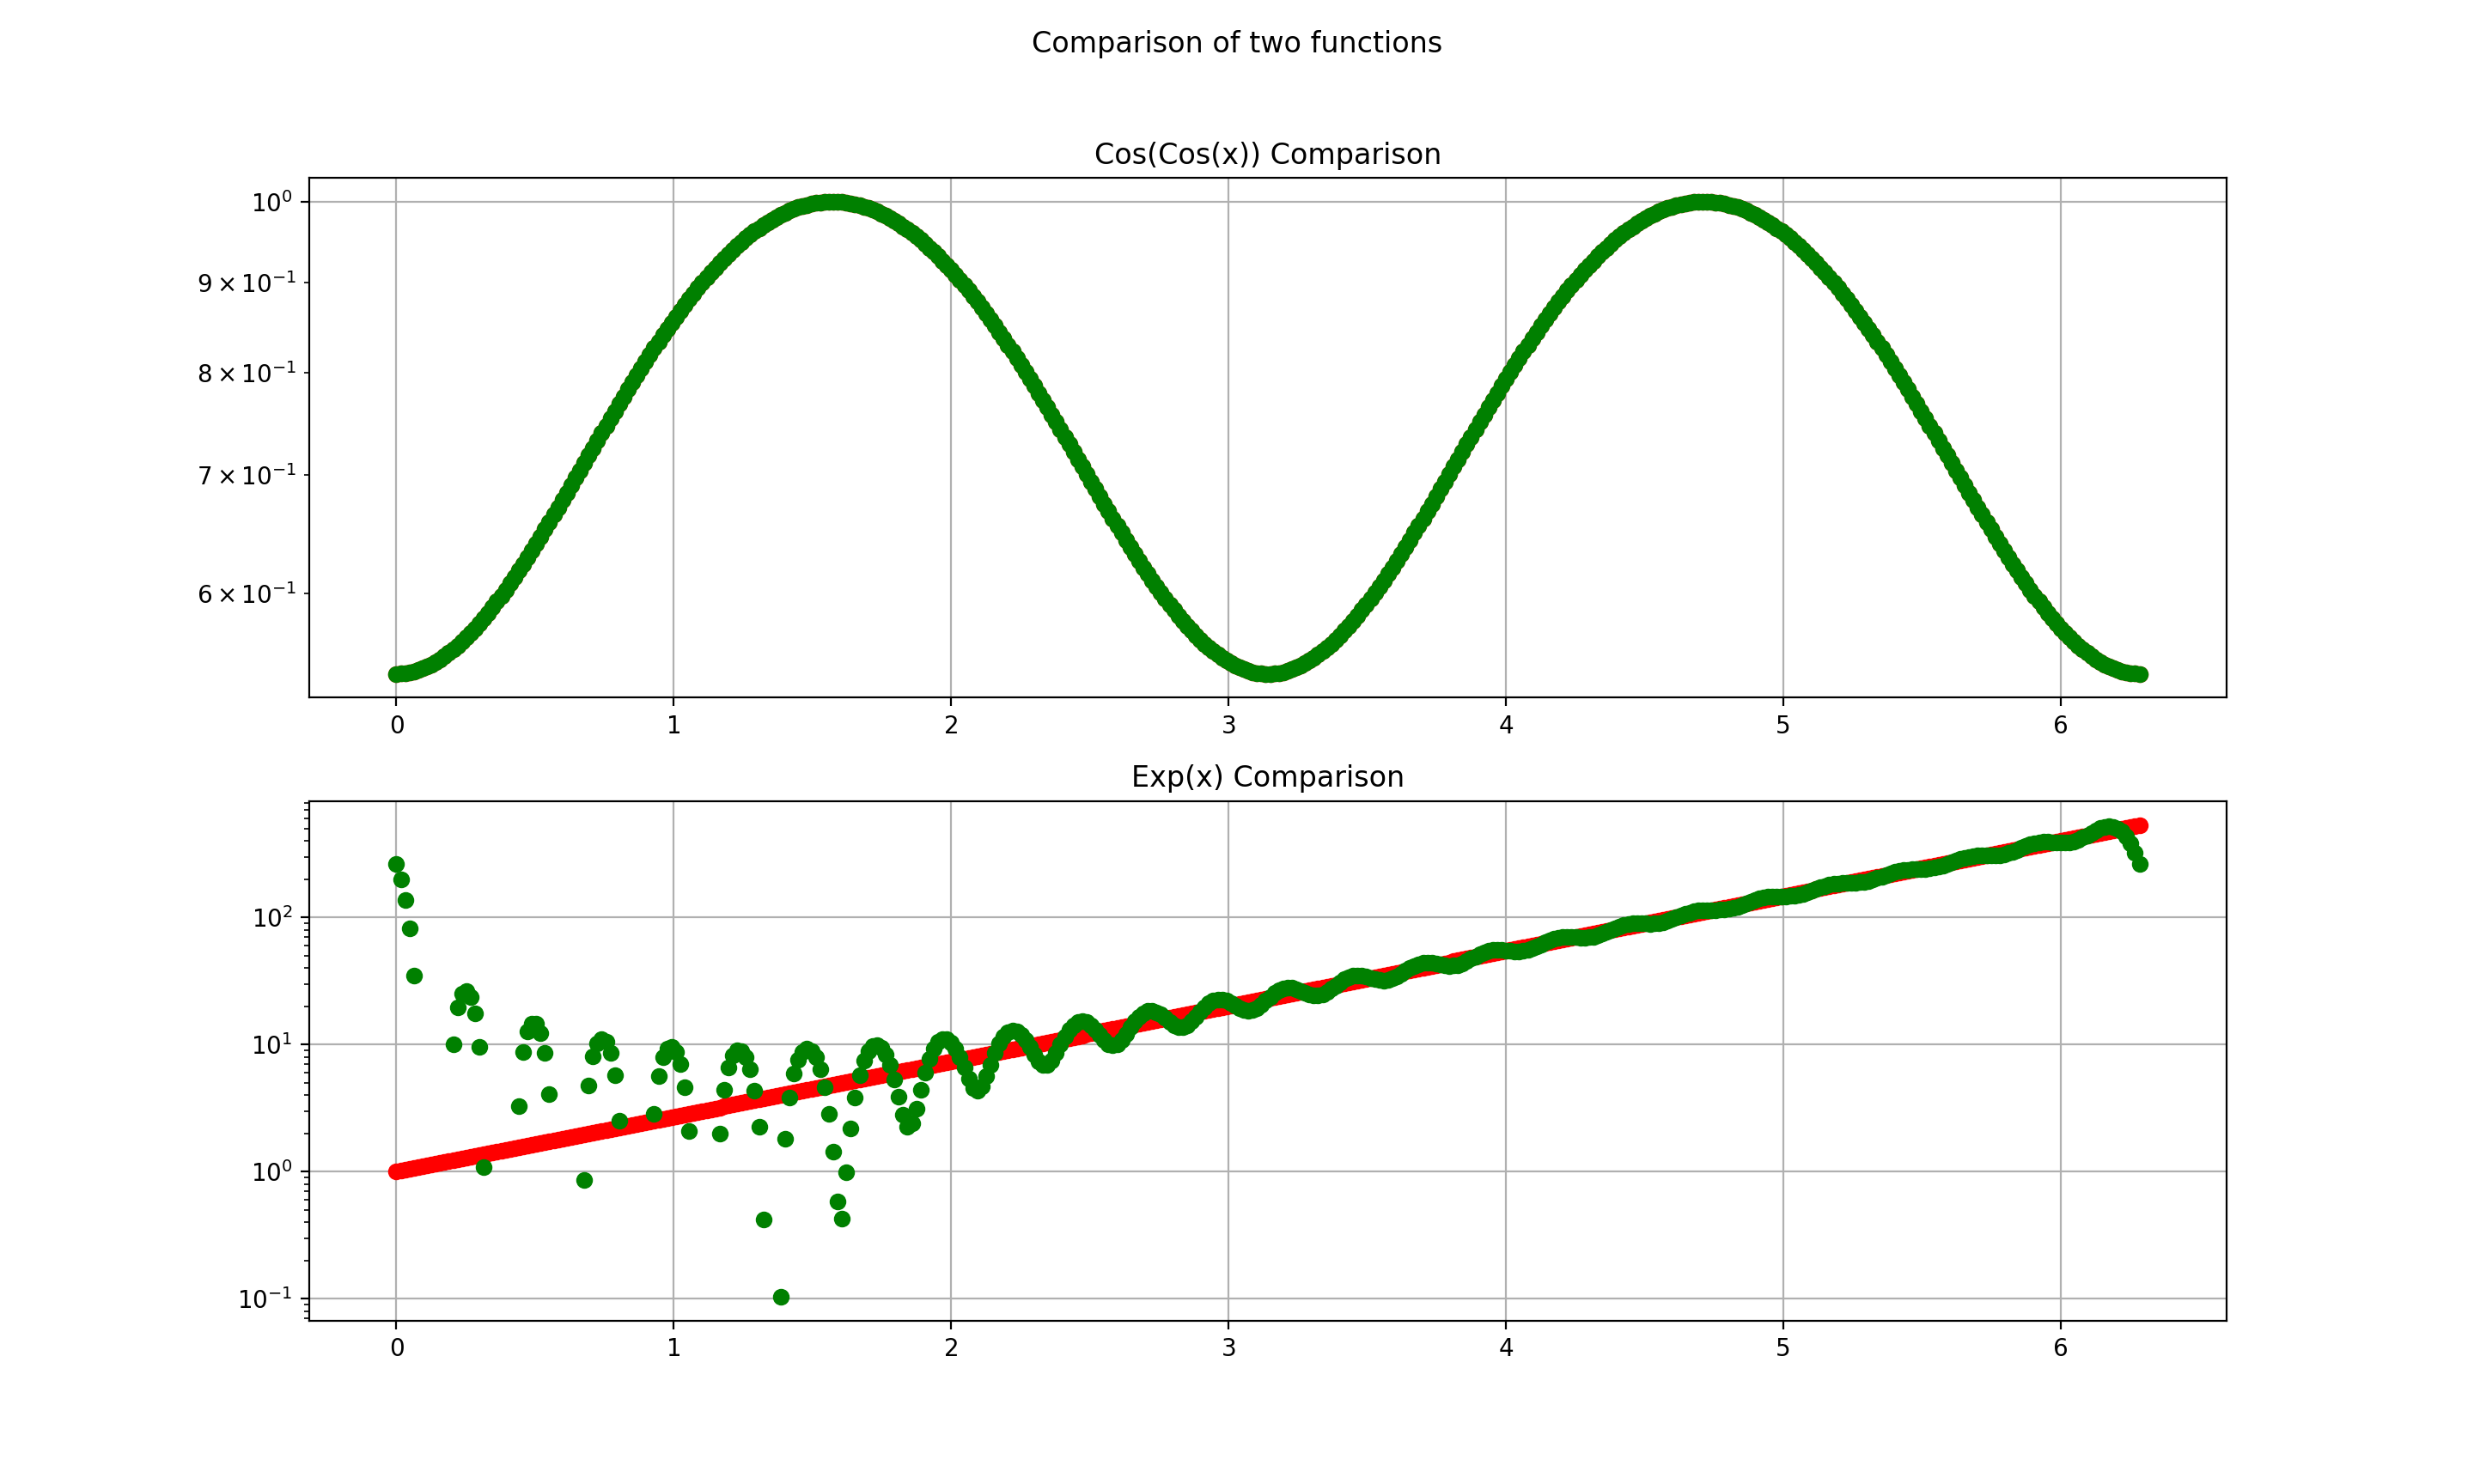
\includegraphics[scale=0.5]{Q6.png}
   	\label{fig:sample}
   \end{figure}
   
   \begin{figure}[!tbh]
   	\centering
   	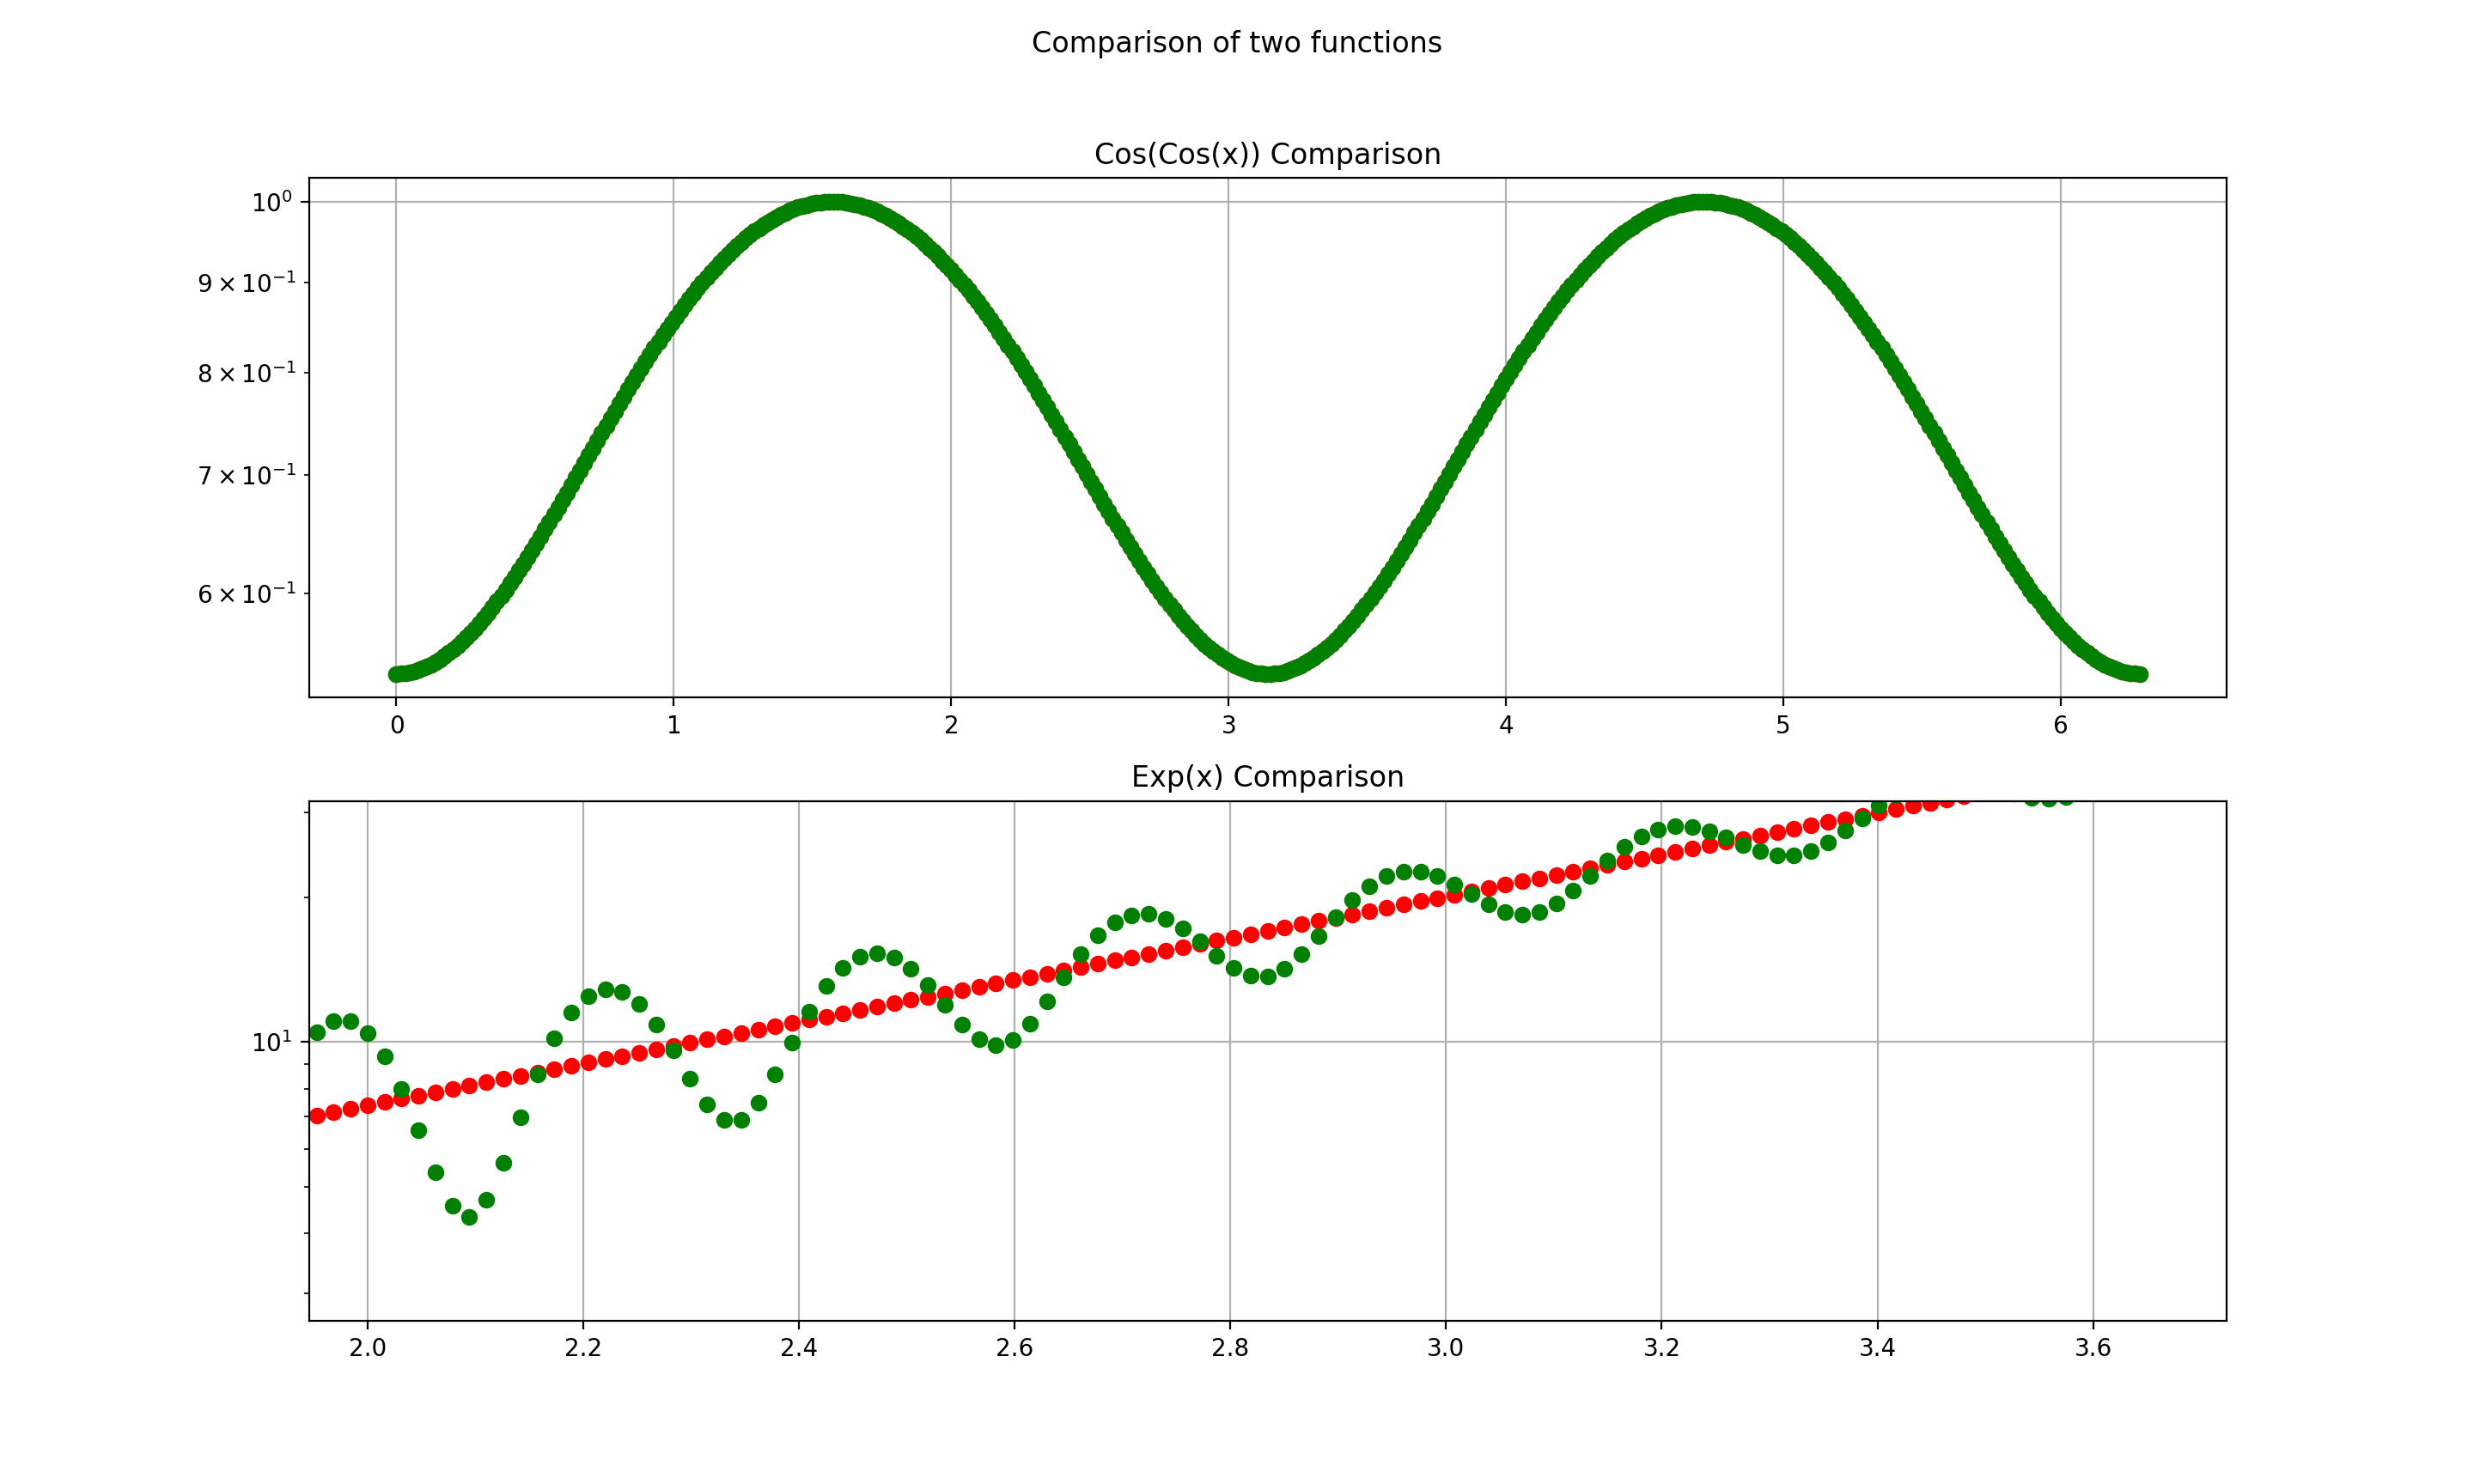
\includegraphics[scale=0.5]{Q6b.png}
	\caption{Zoomed-in Graph}
   	\label{fig:sample}
   \end{figure}
   
\newpage
\section{Conclusions}
\begin{itemize}
   \item  I wrote code in such a way that it finds the first 25 pairs of coefficients of any function if you pass it as argument. I learnt a couple of things about from this code like 
   \begin{itemize}
   	\item A Fourier Series is used to represent any function in a given domain in terms of sum of periodic trigonometric functions of different frequencies.
	\item Fourier Coefficients are decreasing for the function with n as the peak graph in frequency domain goes down
	\item Fourier Coefficients just give the approximate trigonometric estimation of the function, not the accurate unless we take the sum till infinity
	\end{itemize}
 \item Since We tried to approximate $e^x ; [0, 2\pi) $ here, we took it as periodic with period $2\pi$. Since it's non-periodic, there are a lot of non-differentiable points. At these points Fourier approximation(till 25 coefficients) is deviating a lot from actual function.To Summarise, Fourier Series deviates a lot for non-periodic function more than periodic function.
 \item Least Square Method for finding coefficients is faster than integration but is less accurate than latter.
 \item Any function with actual period $2\pi$ will have $b_n$ = 0
 \item \textbf{Gibbs Phenomenon} is the phenomenon due to which the fourier approximations deviate more for non-periodic functions

\end{itemize}
I have learnt how to estimate any function's fourier coefficients using Integration and Least Square Method and checking the accuracy of the function via plotting various graphs.
\end{document}

